\section{Results}
\label{sec:results}

\subsection{RQ1: Does \qss{} Return Complete Evidence Sets, and What Does the Set Formulation Add?}
\label{sec:rq1}

To test whether query-time selection addresses the set problem of Section~\ref{sec:prelim}, we evaluate the selectors without answering on both benchmarks. Table~\ref{tab:select} reports the mean number of opened rounds, full-set recall with the recall of cosine retrieval that opens the same number of rounds for each question (in brackets), the same two quantities on questions with four or more gold rounds, coverage, and the measured selection cost. The same-model controls of Section~\ref{sec:select} separate the set output from relevance judgment and from the recall-oriented instruction, and Figure~\ref{fig:setsize} breaks MemEye recall down by set size.

\begin{table}[t]
\centering
\caption{Set-level retrieval without answering. FSR is full-set recall; brackets give the FSR of cosine retrieval that opens the same number of rounds for each question. The controls use \texttt{gemini-3.8-flash} on the same candidates as \qss{} (MemEye: cosine top-100; MemLens: all rounds). Lightweight selectors use \texttt{gemini-2.5-flash-lite}. Costs are measured.}
\label{tab:select}
\small
\resizebox{\linewidth}{!}{%
\begin{tabular}{lrcccr}
\toprule
Selector & Rounds & FSR [cosine] & FSR, $\ge$4 gold rounds [cosine] & Coverage & \$ / 1k q \\
\midrule
\multicolumn{6}{l}{\textit{MemEye (development; 371 questions, 86 with $\ge$4 gold rounds)}} \\
Cosine top-10 / top-40 & 10 / 40 & 0.633 / 0.922 & 0.279 / 0.779 & 0.774 / 0.959 & 0 \\
\qss{}, full index & 7.3 & \textbf{0.903} [0.539] & \textbf{0.872} [0.151] & 0.943 & 6.43 \\
\qss{}, cosine prefilter $P{=}100$ & 7.7 & 0.919 [0.569] & 0.860 [0.209] & 0.954 & 6.37 \\
\quad Ranking control, cut at the \qss{} size & 7.7 & 0.860 [0.569] & 0.709 [0.209] & -- & 9.51 \\
\quad Ranking control with the \qss{} instruction, same cut & 7.7 & 0.898 [0.569] & 0.814 [0.209] & -- & 9.69 \\
\quad Dynamic cut-off control, grade $\ge$2 & 4.8 & 0.806 [0.445] & 0.686 [0.070] & 0.881 & 10.41 \\
Lightweight selector / with sampling consensus & 9.8 / 10.7 & 0.712 / 0.749 & 0.512 / 0.547 & 0.818 / 0.855 & 0.37 / 1.41 \\
Lightweight selector with resolution write-back & 9.5 & 0.752 [0.606] & 0.558 [0.209] & 0.864 & 0.48 \\
\texttt{gpt-5-mini}, same prompt & 5.9 & 0.728 [0.531] & 0.605 [0.209] & 0.764 & 2.94 \\
\midrule
\multicolumn{6}{l}{\textit{MemLens-32k (held out; 699 questions, 374 with $\ge$4 gold rounds)}} \\
Cosine top-10 / top-40 & 10 / 40 & 0.342 / 0.645 & 0.000 / 0.356 & 0.590 / 0.917 & 0 \\
\qss{}, frozen design & 6.1 & 0.375 [0.176] & 0.043 [0.000] & 0.706 & 6.43 \\
\qss{}, 600-character snippets (declared variant) & 3.9 & 0.286 [0.127] & 0.037 [0.000] & 0.636 & 8.07 \\
\quad Ranking control, cut at the \qss{} size & 6.1 & 0.355 [0.176] & 0.016 [0.000] & -- & 9.95 \\
\quad Ranking control with the \qss{} instruction, same cut & 6.1 & 0.362 [0.176] & 0.019 [0.000] & -- & 9.87 \\
\quad Dynamic cut-off control, grade $\ge$2 & 3.4 & 0.268 [0.130] & 0.008 [0.000] & 0.539 & 10.64 \\
Lightweight selector / with sampling consensus & 5.8 / 6.4 & 0.329 / 0.346 & 0.040 / 0.059 & 0.583 / 0.608 & 0.76 / 0.84 \\
Qwen3-235B-A22B (registered cross-family selector) & 1.4 & 0.149 [0.107] & 0.000 [0.000] & 0.286 & 0.82 \\
\texttt{gpt-5-mini}, same prompt & 7.4 & 0.442 [0.205] & 0.126 [0.016] & 0.684 & 3.63 \\
\bottomrule
\end{tabular}}
\end{table}

First, on MemEye \qss{} reaches a full-set recall of 0.903 while opening 7.3 rounds, whereas cosine retrieval of the same size reaches 0.539 and top-40 retrieval needs 40 rounds to reach 0.922; on sets of four or more rounds the contrast is 0.872 against 0.151. Its recall stays nearly constant across set sizes (0.983, 0.861, 0.868, and 0.900 for 1, 2--3, 4--5, and at least 6 rounds), and its budget follows the set: it opens 3.8 rounds for single-round questions and 26.4 for sets of six or more (Spearman $\rho{=}0.571$ between opened and gold size). Second, the controls decompose the gain of \qss{} over cosine retrieval. Ranking by the same model raises full-set recall over cosine at equal size by $+0.291$ $[+0.240, +0.345]$ on MemEye. Against a ranking instruction that asks only for usefulness, \qss{} appears to add a further $+0.059$ $[+0.032, +0.089]$ ($+0.151$ on sets of four or more rounds), but most of this difference comes from the recall-oriented instruction of \qss{}: when the ranking control receives the same instruction, its recall at the \qss{} size rises from 0.860 to 0.898, and the unordered set adds $+0.022$ $[+0.003, +0.043]$ on MemEye and $+0.013$ $[+0.001, +0.024]$ on MemLens, although the ranking receives the set size of \qss{} for free. The set output therefore matters less for which rounds are found than for how many are opened: without that size, the recall-oriented ranking needs between 10 and 20 rounds on MemEye (0.868 and 0.946) to match the recall that \qss{} reaches with 7.7. Graded relevance with a dynamic cut-off opens fewer rounds and recovers fewer sets on both benchmarks (0.806 and 0.268), because a relevance threshold rejects members that look unremarkable on their own. Third, the absolute recall on MemLens is low for every selector. \qss{} doubles the recall of equal-size cosine retrieval (0.375 against 0.176) but opens 6.1 rounds where the gold set has 5.9 on average and 11.2 for multi-session questions, so wide cosine retrieval recovers more complete sets (0.645 at 40 rounds). The declared variant with longer snippets makes the selector more selective rather than more complete (3.9 rounds at 0.286). The selector from another family behaves inconsistently: \texttt{gpt-5-mini} opens more rounds than the Gemini selector on MemLens but fewer on MemEye. On MemEye histories enlarged 32-fold, a prefilter of 200 keeps the recall at 0.914 with 10.7 rounds (Appendix~\ref{app:results}).

The answer to RQ1 is therefore conditional. Most of the recall of \qss{} comes from model judgment over the whole index and from an instruction calibrated toward recall, while returning an unordered set adds a small further gain and lets the budget follow the size of the set; on MemEye, this yields complete sets with small, adaptive budgets, whereas on MemLens \qss{} improves on equal-size cosine retrieval but under-selects, so that wide similarity retrieval remains more complete. RQ3 relates this difference to how much evidence the index exposes.

\subsection{RQ2: Does Set Recall Improve Answers on the Development Benchmark?}
\label{sec:rq2}

To test whether better retrieval reaches the answer, we run the full pipeline on all 371 MemEye questions with both readers. Table~\ref{tab:e2e} reports accuracy, paired differences from top-40 retrieval and from full-context reading, opened rounds, and cost, measured and, for \qss{}, estimated with a warm index cache. Figure~\ref{fig:cost} places the main conditions on an accuracy--cost plane, and Table~\ref{tab:cluster} in the appendix repeats the main contrasts under a two-stage bootstrap over scenarios.

\begin{table}[t]
\centering
\caption{End-to-end accuracy on MemEye (371 questions; development benchmark). $\Delta$ columns give paired differences with 95\% question-level bootstrap intervals. Cost is the spend per 1k questions over all calls except the judge: measured, and after the slash estimated with the static index served from the prefix cache (Appendix~\ref{app:cost}).}
\label{tab:e2e}
\small
\resizebox{\linewidth}{!}{%
\begin{tabular}{llrcccr}
\toprule
Reader & Method & Rounds & Accuracy & $\Delta$ vs.\ RAG@40 & $\Delta$ vs.\ FC & \$ / 1k q \\
\midrule
\multirow{7}{*}{\shortstack[l]{2.5-flash-lite\\(no thinking)}}
 & Full context (FC) & 126.5 & 0.495 & $+0.007$ & -- & 0.37 \\
 & RAG@40 & 38.7 & 0.488 & -- & $-0.007$ & 0.86 \\
 & Annotated evidence & 2.8 & 0.539 & $+0.051$ & $+0.044$ & 0.17 \\
 & \qss{} & 7.3 & \textbf{0.541} & $+0.053$ $[+0.009, +0.098]$ & $+0.046$ $[+0.001, +0.092]$ & 6.73 / 2.20 \\
 & Dynamic cut-off control & 4.8 & 0.509 & $+0.021$ $[-0.022, +0.064]$ & $+0.013$ & 10.63 \\
 & Union of \qss{} and cosine top-20 & 22.4 & 0.472 & $-0.015$ & $-0.023$ & 7.12 \\
 & Lightweight selector, consensus + write-back & 10.0 & 0.518 & $+0.030$ $[-0.011, +0.072]$ & $+0.023$ & 1.86 \\
\midrule
\multirow{3}{*}{\shortstack[l]{2.5-flash-lite\\(thinking 1,024)}}
 & Full context (FC) & 126.5 & 0.571 & $+0.019$ & -- & 0.67 \\
 & RAG@40 & 38.7 & 0.552 & -- & $-0.019$ & 1.12 \\
 & \qss{} & 7.3 & \textbf{0.597} & $+0.045$ $[+0.003, +0.086]$ & $+0.026$ $[-0.019, +0.073]$ & 6.97 / 2.39 \\
\midrule
\multirow{7}{*}{3.8-flash}
 & Full context (FC) & 126.5 & \textbf{0.819} & $+0.079$ & -- & 8.97 \\
 & RAG@40 & 38.7 & 0.741 & -- & $-0.079$ & 10.00 \\
 & Annotated evidence & 2.8 & 0.746 & $+0.005$ & $-0.073$ & 2.76 \\
 & \qss{} & 7.3 & 0.761 & $+0.020$ $[-0.014, +0.055]$ & $-0.059$ & 10.27 / 5.80 \\
 & \qss{}, index as context & 7.3 & 0.796 & $+0.055$ $[+0.021, +0.089]$ & $-0.024$ $[-0.050, +0.002]$ & 15.70 / 6.80 \\
 & Dynamic cut-off control & 4.8 & 0.759 & $+0.018$ $[-0.020, +0.055]$ & $-0.061$ & 13.50 \\
 & Union of \qss{} and cosine top-40 & 39.7 & 0.771 & $+0.030$ $[-0.003, +0.063]$ & $-0.049$ & 16.42 \\
\bottomrule
\end{tabular}}
\end{table}

\begin{figure}[t]
\centering
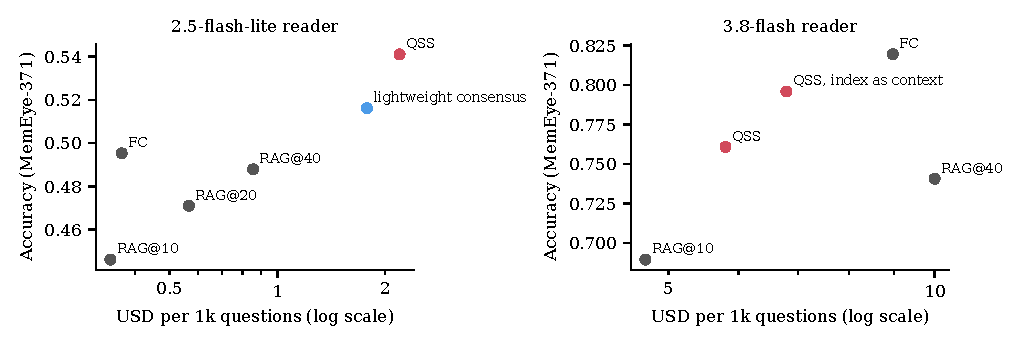
\includegraphics[width=0.92\linewidth]{figures/cost.pdf}
\caption{Accuracy against cost per 1,000 MemEye questions (log scale) for the lightweight reader without thinking (left) and the strong reader (right). Points for \qss{} use the warm-cache estimate; all other points are measured.}
\label{fig:cost}
\end{figure}

First, with the lightweight reader, \qss{} raises accuracy from 0.488 (top-40) and 0.495 (full context) to 0.541, the accuracy of the same reader on the annotated evidence, and it keeps a lead of $+0.045$ over top-40 retrieval when the reader thinks. The lightweight reader needs a set that is both complete and small: the dynamic cut-off control opens fewer rounds and falls 0.032 $[-0.065, -0.001]$ below \qss{}, and the union of \qss{} with cosine top-20 is complete in 97.3\% of questions but falls 0.069 $[-0.111, -0.027]$ below \qss{} because the added rounds distract the reader. Second, with the strong reader, the selected set alone yields $+0.020$ $[-0.014, +0.055]$ over top-40 retrieval and matches the dynamic cut-off control, whereas the index-as-context variant reaches 0.796 ($+0.055$ $[+0.021, +0.089]$), within 0.024 of full-context reading while opening 7.3 instead of 126.5 rounds; the strong reader thus profits from the narrative framing of the index, which the lightweight reader does not use ($-0.019$). Third, the robustness checks separate the claims. Under the two-stage bootstrap over the eight scenarios, the strong-reader gain of the index-as-context variant keeps an interval above zero ($[+0.004, +0.126]$, six of eight scenarios positive), whereas the lightweight-reader gain does not ($[-0.014, +0.120]$, six of eight positive); the retrieval gain over equal-size cosine is positive in all eight scenarios. An independent judge from another family preserves every ordering and gives $+0.057$ $[+0.012, +0.102]$ and $+0.044$ $[+0.012, +0.080]$ for the two main contrasts. Finally, the cost of \qss{} depends on caching: the strong pipeline with index context costs \$15.7 per 1,000 questions as measured here, and \$7.0 when the static index is served from an explicit context cache (Section~\ref{sec:rq6}); full-context reading remains the most accurate option for the strong reader on histories that fit in context.

On the development benchmark, complete evidence sets therefore improve answers, and this conclusion is most reliable for the strong reader with the index as context. For the lightweight reader, the gain is consistent across judges and readers but not established at the level of scenarios; Appendix~\ref{app:results} adds the scale test and Mem-Gallery, where the benefit grows with history length and vanishes on a benchmark that wide top-$k$ already serves well.

\subsection{RQ3: Do the Gains Hold on a Held-Out Benchmark?}
\label{sec:rq3}

To test whether the conclusions generalize beyond the data on which we developed the method, we evaluate the registered conditions on MemLens. Table~\ref{tab:memlens} reports accuracy under the official judge for the lightweight reader on all 699 questions, for the strong reader on a fixed subset of 200 questions, and for the lightweight reader on the same subset at the 128k context length. The registered hypotheses were that \qss{} recovers more complete sets than equal-size cosine retrieval (H1), improves answers over top-40 retrieval with the lightweight reader (H2), matches or beats the dynamic cut-off control (H3), keeps its accuracy from 32k to 128k while full-context reading degrades (H4), and that a selector from another family beats equal-size cosine retrieval (H5). Rows marked as post hoc in Table~\ref{tab:memlens} were added after the registered runs.

\begin{table}[t]
\centering
\caption{Held-out end-to-end accuracy on MemLens under the official judge prompt (Qwen3-VL-235B-A22B; a \texttt{gemini-3.8-flash} judge agrees on 96--97\% of answers). $\Delta$ gives paired differences from RAG@40 with 95\% bootstrap intervals. Costs are measured; every question has its own haystack, so no index is cached across questions. Rows marked post hoc were not part of the registration.}
\label{tab:memlens}
\small
\begin{tabular}{llrccr}
\toprule
Setting & Method & Rounds & Accuracy & $\Delta$ vs.\ RAG@40 & \$ / 1k q \\
\midrule
\multirow{11}{*}{\shortstack[l]{32k, 2.5-flash-lite\\(699 questions)}}
 & Full context (FC) & 64.6 & 0.454 & $-0.020$ $[-0.046, +0.004]$ & 3.06 \\
 & RAG@20 & 20.0 & 0.458 & $-0.016$ & 0.79 \\
 & RAG@40 & 40.0 & 0.474 & -- & 1.74 \\
 & Annotated evidence & 5.9 & 0.496 & $+0.023$ $[-0.007, +0.053]$ & 0.46 \\
 & \qss{}, frozen design & 6.1 & 0.484 & $+0.010$ $[-0.020, +0.040]$ & 6.84 \\
 & \qss{}, 600-character snippets & 3.9 & \textbf{0.502} & $+0.029$ $[-0.001, +0.059]$ & 8.36 \\
 & Dynamic cut-off control & 3.4 & 0.474 & $+0.000$ $[-0.033, +0.031]$ & 10.89 \\
 & Lightweight selector, consensus & 6.4 & 0.448 & $-0.026$ $[-0.056, +0.003]$ & 1.26 \\
 & Qwen3-235B-A22B selector & 1.4 & 0.313 & $-0.160$ $[-0.197, -0.124]$ & 0.96 \\
 & \texttt{gpt-5-mini} selector (post hoc) & 7.4 & 0.449 & $-0.024$ $[-0.053, +0.003]$ & 4.08 \\
 & Union of \qss{} and cosine top-20 (post hoc) & 21.5 & 0.474 & $+0.000$ $[-0.024, +0.024]$ & 7.31 \\
\midrule
\multirow{5}{*}{\shortstack[l]{32k, 3.8-flash\\(200 questions)}}
 & Full context (FC) & 64.8 & 0.725 & $-0.030$ $[-0.075, +0.010]$ & 24.98 \\
 & RAG@40 & 40.0 & \textbf{0.755} & -- & 14.83 \\
 & Annotated evidence & 5.8 & 0.730 & $-0.025$ $[-0.070, +0.020]$ & 4.66 \\
 & \qss{}, frozen design & 6.0 & 0.675 & $-0.080$ $[-0.135, -0.030]$ & 10.70 \\
 & \qss{}, index as context & 6.0 & 0.670 & $-0.085$ $[-0.140, -0.035]$ & 16.16 \\
\midrule
\multirow{4}{*}{\shortstack[l]{128k, 2.5-flash-lite\\(same 200 questions)}}
 & Full context (FC) & 245.0 & 0.440 & $-0.035$ $[-0.100, +0.030]$ & 11.65 \\
 & RAG@40 & 40.0 & 0.475 & -- & 1.16 \\
 & Annotated evidence & 5.8 & 0.500 & $+0.025$ $[-0.040, +0.090]$ & 0.45 \\
 & \qss{}, frozen design & 6.6 & \textbf{0.505} & $+0.030$ $[-0.030, +0.090]$ & 21.75 \\
\bottomrule
\end{tabular}
\end{table}

First, H1 holds at the level of retrieval (Table~\ref{tab:select}) and H3 holds end to end (0.484 against 0.474 for the dynamic cut-off control, at lower cost), but H2 does not hold: with the lightweight reader, the frozen \qss{} is only $+0.010$ $[-0.020, +0.040]$ above top-40 retrieval. The declared variant with longer snippets reaches 0.502, the best accuracy in the table and above the annotated evidence, but its interval still touches zero ($+0.029$ $[-0.001, +0.059]$); the dynamic cut-off control, the union with cosine top-20, sampling consensus, and both selectors from other families do not exceed top-40 retrieval. H5 holds only formally: the registered Qwen3-235B-A22B selector beats equal-size cosine retrieval (0.149 against 0.107) while returning 1.4 rounds on average, and its answers fall to 0.313. By question type, \qss{} gains on multi-session reasoning (0.252 against 0.189) and information extraction and loses on temporal reasoning and knowledge updates (Appendix Table~\ref{tab:memlens_type}). Second, with the strong reader, \qss{} is 0.080 $[-0.135, -0.030]$ below top-40 retrieval, and adding the index as context does not help. Even the annotated evidence falls below top-40 retrieval for this reader (0.730 against 0.755), which indicates that the annotations omit context that a strong reader exploits, so any focused selection is capped below wide retrieval on this benchmark. Third, at 128k, full-context reading with the lightweight reader changes little (0.450 on the same 200 questions at 32k against 0.440), so H4 is only weakly supported, and \qss{} stays at the level of top-40 retrieval while its selection cost rises with the longer index. Index visibility accounts for much of the contrast with MemEye. In MemEye, 95\% of the question words that occur in gold rounds are visible in their index lines; in MemLens only 37\% are, because gold user messages are long (median 532 characters against 45) and the evidence is typically an aside in a conversation about another topic, accompanied by a generically captioned photo. The declared variant raises visibility to 63\% and improves accuracy by 0.018 over the frozen design, yet it makes the selector open fewer rounds. Fourth, three analyses test this explanation and the gold sets behind it (Appendix Table~\ref{tab:visibility}). Masking every content word of the question in all index lines of MemEye, with everything else fixed, lowers the full-set recall of \qss{} by 0.089 $[-0.124, -0.054]$ and the accuracy of the lightweight reader with thinking by 0.086 $[-0.127, -0.045]$, to 0.511, which is below top-40 retrieval with thinking (0.552); masking half of these words costs only 0.024 of recall because the selector opens more rounds. Hiding the evidence from the index thus reproduces the MemLens pattern on MemEye, although the selector partly compensates through other cues. The 600-character lines explain the apparent conflict between visibility and recall: they raise the full-set recall of the rounds with evidence turns from 0.614 to 0.828 but lower that of the rounds with evidence images from 0.251 to 0.133, because the selector stops once the textual evidence is visible and misses the image rounds whose captions remain generic. Finally, the advantage over equal-size cosine retrieval holds under every gold definition that we tested, namely evidence-turn rounds (0.614 against 0.385), evidence-image rounds (0.251 against 0.106), and coverage of the answer sessions (0.687 against 0.554). Among the 13 subset questions on which the strong reader is right with top-40 retrieval but wrong with the annotated evidence, top-40 retrieval also returned other rounds of an answer session in all 13 cases and the answer words in non-gold rounds in 6, so the derived gold omits context of the answer sessions.

The answer to RQ3 is negative for the general claim and positive for a conditional one. On held-out data with low index visibility, query-time set selection does not improve answers over wide similarity retrieval for a lightweight reader and hurts a strong reader, even though it still recovers more complete sets than equal-size cosine retrieval; because the MemLens annotations omit context that the strong reader uses, full-set recall is only a partial account of this outcome. Its benefit on MemEye depends on an index that exposes the evidence, as the masking experiment shows, and on a reader that profits from a small input.

\subsection{RQ4: Where Does the Selection Capability Reside, and Does It Transfer?}
\label{sec:rq4}

The gap between selectors raises the question of what the developed selector does that other mechanisms cannot. We test three hypotheses with selection-only experiments on MemEye: the capability is information that could be written into the memory at ingestion; it is a matter of prompting or task structure that a lightweight model can follow; or it depends on the selector model. Table~\ref{tab:ablate} reports full-set recall and opened rounds for each intervention; the lightweight variants are exploratory, and we report every variant that we evaluated.

\begin{table}[t]
\centering
\caption{Where the set-selection capability resides (MemEye, selection only). Brackets give the FSR of cosine retrieval with the same per-question size where the size varies strongly. Rows marked $^\ddagger$ use a fixed random subset of 150 questions, on which \texttt{gemini-3.8-flash} reaches 0.887 with 7.7 rounds. The lightweight model is \texttt{gemini-2.5-flash-lite}; it reaches 0.712 with 9.8 rounds without interventions.}
\label{tab:ablate}
\small
\resizebox{\linewidth}{!}{%
\begin{tabular}{llrc}
\toprule
Hypothesis & Intervention & Rounds & FSR \\
\midrule
\multirow{7}{*}{\shortstack[l]{Selector model\\(same prompt and index)}}
 & \texttt{gemini-3.8-flash} (\qss{}) & 7.3 & 0.903 \\
 & \texttt{gemini-3.5-flash-lite} / \texttt{gemini-3.1-flash-lite} & 3.9 / 4.3 & 0.685 / 0.660 \\
 & \texttt{gemini-2.5-flash-lite}, without / with a 2,048-token thinking budget & 9.8 / 4.6 & 0.712 / 0.636 \\
 & \texttt{gpt-5-mini} & 5.9 & 0.728 \\
 & \texttt{gpt-5}$^\ddagger$ & 2.8 & 0.573 \\
 & Qwen3-235B-A22B, thinking$^\ddagger$ & 2.3 & 0.407 \\
 & Qwen3-235B-A22B, instruction (mostly empty selections) & 1.5 & 0.264 \\
\midrule
\multirow{3}{*}{\shortstack[l]{Write-time knowledge\\(strong model at ingestion)}}
 & Named groups written once; lightweight selector picks groups (+ cosine top-5) & 22.1 (23.2) & 0.636 (0.717) \\
 & Predicted aliases added to the index; lightweight selector & 9.3 & 0.736 \\
 & Predicted aliases added to cosine keys (top-10 / top-40) & 10 / 40 & 0.642 / 0.933 \\
\midrule
\multirow{5}{*}{\shortstack[l]{Prompting and structure\\(lightweight selector)}}
 & Count the groups first, then list members & 8.1 & 0.663 \\
 & Decompose into membership predicates, verify per predicate & 8.7 & 0.617 \\
 & Narrative coordinates and session headers in the index & 10.0 & 0.690 \\
 & Three demonstrations of strong selections from other scenarios & 8.8 & 0.639 \\
 & Chunked exhaustive scan (30 rounds per call) & 18.4 & 0.765 [0.782] \\
\midrule
\multirow{4}{*}{\shortstack[l]{Partial remedies\\(lightweight selector)}}
 & Union of five sampled selections & 15.2 & 0.836 [0.714] \\
 & Resolution write-back of resolutions that the selector itself produced & 9.7 & 0.725 \\
 & Resolution write-back of strong resolutions for 30\% / 100\% of questions & 9.5 / 9.5 & 0.741 / 0.752 \\
 & Model-free reuse of resolved sets + cosine top-5 & 19.1 & 0.836 [0.787] \\
\bottomrule
\end{tabular}}
\end{table}

First, the capability is not information that the write-time organizations we tested can supply. When the strong model groups each history once into named sets, the groups come out at the level of sessions or topics, and a lightweight selector that picks groups opens 22.1 rounds with a full-set recall of 0.636, because the sets that questions refer to cut across these groups; predicted aliases barely change cosine recall (0.633 to 0.642 at top-10) and lift the lightweight selector only from 0.712 to 0.736. Second, prompting and structure do not transfer it to the lightweight selector: counting groups first, predicate decomposition, narrative coordinates, and demonstrations leave it at or below its unaided recall, a thinking budget makes it open fewer rounds, and chunked scanning stays below cosine retrieval of the same size. Its failures are wrong members rather than too few: on failures it opens 11.1 rounds for 4.3 gold rounds. Third, the selection behavior does not transfer across model families with the same prompt. \texttt{gpt-5-mini} reaches 0.728 with 5.9 rounds, while \texttt{gpt-5} and the thinking version of Qwen3-235B-A22B return only two or three rounds and recover 0.573 and 0.407 of the sets on the subset, and the instruction version mostly returns empty selections. Larger or reasoning-oriented models are thus not better set selectors by default. The instruction to include every possible member appears to compete with a preference for precise answers, and the prompt that we developed with Gemini does not calibrate these models. Two remedies recover part of the gap for the lightweight selector. Sampling consensus with two votes keeps 10.7 rounds at 0.749 recall, and resolution write-back reaches 0.752 with strong resolutions of earlier questions, 0.741 when only 30\% of earlier questions were resolved by the strong selector, and 0.725 when the lightweight selector writes back its own resolutions.

These results indicate that, on MemEye, set selection depends on query-time reasoning that is calibrated toward recall; neither the write-time organizations we tested nor structural prompting reproduce it, and it varies more with model family and prompt calibration than with model size. Writing resolutions back into the memory amortizes part of it, but end to end the lightweight remedies gain only 0.02 to 0.03 over top-40 retrieval, with intervals that include zero (Table~\ref{tab:e2e}).

\subsection{RQ5: Can the Diagnosis Be Turned into a Better Mechanism?}
\label{sec:rq5}

The held-out test located two failures, index lines that hide the evidence and lightweight readers that fail to aggregate complete sets, and we asked whether a mechanism derived from them improves answers on data that played no role in its design. We first analyzed the stored outputs without new calls, then explored mechanisms on MemEye and the MemLens development part, and finally evaluated the selected configurations once on the 466 MemLens test questions under a registration written before the run. Table~\ref{tab:p5dev} reports the development results of the lightweight reader, Table~\ref{tab:p5test} reports the registered test, and Table~\ref{tab:wma} reports a second registered test on the external WorldMemArena benchmark with the design frozen. Its primary hypothesis was that VGS beats top-40 retrieval with the lightweight reader; the secondary hypotheses concerned a cheaper variant that replaces the low-visibility path by cosine top-20 with notes (VGS-cheap), the contribution of the notes, a comparison with top-40 retrieval with thinking, and the 600-character selection with the strong reader.

\begin{table}[t]
\centering
\caption{Mechanism exploration on development data with the lightweight reader (\texttt{gemini-2.5-flash-lite}): MemEye (371 questions) and the MemLens development part (233 questions). Notes are written per selected round by \texttt{gemini-2.5-flash-lite}; cost is the measured spend per 1k MemLens questions.}
\label{tab:p5dev}
\small
\begin{tabular}{lccr}
\toprule
Mechanism & MemEye & MemLens dev & \$ / 1k q \\
\midrule
RAG@40 & 0.488 & 0.489 & 1.77 \\
RAG@40 with a 1,024-token thinking budget & \textbf{0.552} & 0.515 & 1.99 \\
\qss{}, 200-character index lines & 0.541 & 0.485 & 6.83 \\
\quad + session closure (all rounds of the selected sessions) & 0.526 & 0.476 & 7.21 \\
\qss{}, model-written gist instead of the snippet & 0.504 & 0.515 & 7.15 \\
\qss{}, 600-character index lines & 0.528 & 0.549 & 8.32 \\
\quad + session closure & -- & 0.472 & 8.86 \\
\quad + per-member notes & 0.517 & \textbf{0.562} & 8.83 \\
Cosine top-20 + per-member notes & 0.471 & 0.536 & 2.47 \\
Sentence-granular top-20 & -- & 0.489 & 0.97 \\
VGS (gate $\tau{=}0.7$) & 0.541 & 0.558 & 8.60 \\
\bottomrule
\end{tabular}
\end{table}

\begin{table}[t]
\centering
\caption{Registered held-out test on the MemLens test part (466 questions; official judge). $\Delta$ gives paired differences from RAG@40 with 95\% bootstrap intervals. VGS-cheap replaces the low-visibility path by cosine top-20 with notes; VGS-strong uses the strong reader without notes. Costs are measured (one haystack per question, no index cache).}
\label{tab:p5test}
\small
\begin{tabular}{llccr}
\toprule
Reader & Method & Accuracy & $\Delta$ vs.\ RAG@40 & \$ / 1k q \\
\midrule
\multirow{8}{*}{2.5-flash-lite}
 & RAG@40 & 0.466 & -- & 1.73 \\
 & RAG@40 with thinking & 0.496 & $+0.030$ $[-0.013, +0.073]$ & 1.94 \\
 & \qss{}, 200-character lines & 0.483 & $+0.017$ $[-0.019, +0.054]$ & 6.84 \\
 & \qss{}, 600-character lines & 0.479 & $+0.013$ $[-0.024, +0.049]$ & 8.38 \\
 & \qss{}, 600-character lines + notes & 0.536 & $+0.071$ $[+0.032, +0.109]$ & 8.88 \\
 & Cosine top-20 + notes & 0.485 & $+0.019$ $[-0.019, +0.058]$ & 2.50 \\
 & VGS & \textbf{0.536} & $+0.071$ $[+0.032, +0.109]$ & 8.63 \\
 & VGS-cheap & 0.494 & $+0.028$ $[-0.011, +0.069]$ & 3.08 \\
\midrule
\multirow{4}{*}{3.8-flash}
 & RAG@40 & \textbf{0.689} & -- & 14.74 \\
 & \qss{}, 200-character lines & 0.618 & $-0.071$ $[-0.107, -0.034]$ & 10.79 \\
 & \qss{}, 600-character lines & 0.659 & $-0.030$ $[-0.062, +0.002]$ & 11.35 \\
 & VGS-strong & 0.655 & $-0.034$ $[-0.069, -0.002]$ & 11.21 \\
\bottomrule
\end{tabular}
\end{table}

\begin{table}[t]
\centering
\caption{Registered external test on WorldMemArena lifelong-personal (1,100 questions; design frozen; MemEye rubric judge), corrected run with benchmark image identifiers (see text). $\Delta$ gives paired differences from RAG@40 with the same reader and 95\% bootstrap intervals. Costs are measured and include the creation and storage of the context caches.}
\label{tab:wma}
\small
\begin{tabular}{llccr}
\toprule
Reader & Method & Accuracy & $\Delta$ vs.\ RAG@40 & \$ / 1k q \\
\midrule
\multirow{4}{*}{2.5-flash-lite} & RAG@40 & 0.779 & -- & 1.17 \\
 & \qss{}, cached index & 0.791 & $+0.012$ $[-0.005, +0.028]$ & 4.30 \\
 & \qss{}, 600-character lines + notes & 0.785 & $+0.005$ $[-0.013, +0.023]$ & 6.47 \\
 & VGS & 0.786 & $+0.007$ $[-0.011, +0.025]$ & 6.42 \\
\midrule
\multirow{2}{*}{3.8-flash} & RAG@40 & 0.889 & -- & 8.89 \\
 & \qss{} with index, cached index & 0.882 & $-0.007$ $[-0.018, +0.005]$ & 10.21 \\
\bottomrule
\end{tabular}
\end{table}

First, the failure analysis showed that reading, not retrieval, limits the lightweight reader. Given the complete annotated evidence, it answers 6\% of the MemLens arithmetic questions and 9\% of the counting questions, against 67\% and 91\% for the strong reader on the 200-question subset, and on MemEye its accuracy with complete \qss{} sets falls from 0.64 to 0.45 as the set grows from one to four or more rounds. Second, mechanisms that complete the set more aggressively did not help. Closing the set selected with 600-character index lines over its sessions raises full-set recall on the MemLens development part from 0.292 to 0.824, yet accuracy falls from 0.549 to 0.472, because the additional rounds distract the reader. Member expansion by image or text similarity, expansion of the question into concrete instances, and a sentence-granular index did not improve retrieval consistently across the two benchmarks, and none of them improved answers; index lines whose snippet is replaced by a model-written gist of the message lost the exact wording that MemEye questions use. Third, two changes helped on low-visibility data only. Longer index lines and per-member notes raise the MemLens development accuracy to 0.562, whereas both slightly lower the MemEye accuracy (0.528 and 0.517 against 0.541); routing each question by its estimated visibility lets VGS keep the MemEye accuracy of \qss{} and reach 0.558 on the MemLens development part. Fourth, the registered test supports the primary hypothesis: VGS improves the lightweight reader by $+0.071$ $[+0.032, +0.109]$ over top-40 retrieval, and the notes add $+0.058$ $[+0.021, +0.097]$ over the same selection without notes. The gains concentrate where the failure analysis predicted them: arithmetic rises from 0.03 to 0.21, counting from 0.10 to 0.23, and ordering from 0.12 to 0.38, while date extraction drops from 0.98 to 0.94. Within the test part, the gain also follows the visibility estimate rather than only the benchmark: the 407 questions below the threshold gain $+0.084$ $[+0.042, +0.125]$, whereas on the 59 questions above it, where VGS keeps plain \qss{}, the notes path would not have helped (0.542 for both paths against 0.559 for top-40 retrieval), and across the 699 MemLens questions the estimate $\hat{v}(q)$ correlates with the oracle index visibility (Spearman 0.48; AUC 0.75 for an oracle visibility of at least 0.5). VGS is $+0.041$ $[-0.002, +0.084]$ above top-40 retrieval with thinking, which supports this comparison only weakly, and two development gains did not replicate, namely longer index lines alone ($+0.060$ on development data and $+0.013$ on the test) and notes over a wide cosine pool, so that VGS-cheap gains only $+0.028$ $[-0.011, +0.069]$ at 1.8 times the cost of top-40 retrieval. For the strong reader, wide retrieval remains best: the 600-character selection is $-0.030$ $[-0.062, +0.002]$ below top-40 retrieval, and VGS-strong is significantly worse ($-0.034$ $[-0.069, -0.002]$). On Mem-Gallery, where 87.7\% of the questions take the high-visibility path, VGS equals \qss{} (0.852 against 0.839 for top-40 retrieval), and its low-visibility subset gains nothing from the notes (0.876 against 0.878). The low-visibility path costs \$8.88 per 1,000 MemLens questions, of which \$8.10 is the strong selection call. Fifth, the external test does not confirm the gain. In the registered run, our loader labelled images by round rather than by the identifiers of the benchmark, which made its visual-search questions unanswerable for every method; Table~\ref{tab:wma} reports the corrected run, and the registered run leads to the same conclusions (VGS $+0.003$, \qss{} $+0.009$). WorldMemArena has a visibility estimate as low as MemLens (mean 0.438 against 0.427), so VGS takes the notes path for 97\% of its questions, yet VGS is only $+0.007$ $[-0.011, +0.025]$ above top-40 retrieval, and \qss{} alone is $+0.012$ $[-0.005, +0.028]$. Two differences from MemLens may explain this outcome. The lightweight reader already reaches 0.779 on these questions with top-40 retrieval, against 0.466 on MemLens, and the notes path opens 10.5 rounds and writes 16.0 notes per question, against 3.9 rounds and 3.7 notes on MemLens, so the notes summarize many members for a reader that already performs well without them. Most questions also need little visual information: without any image or description, top-40 retrieval still reaches 0.699, which is 90\% of its accuracy, whereas on MemEye full-context reading without visual information keeps 23\% of the accuracy of the strong reader. The selection itself still transfers: \qss{} touches every evidence session for 0.739 of the questions, against 0.689 for cosine retrieval of the same size ($+0.050$ $[+0.031, +0.070]$).

The answer to RQ5 is positive for lightweight readers on MemLens and negative beyond it. Turning the diagnosis into a decision, namely to compensate for low index visibility with wider index lines and with notes that make the set explicit for the reader, yields a gain that holds on held-out MemLens questions, whereas making the set more complete without helping the reader use it does not. On an external benchmark with equally low visibility, the same frozen design gains no significant accuracy, so low visibility alone does not identify the questions that notes help; on MemLens, the gain coincides with a reader that fails to aggregate a few members. Strong readers do not benefit on either benchmark, and the gain requires a strong selection call per question, whose cost RQ6 examines.

\subsection{RQ6: Can Set Selection Approach the Cost of Retrieval?}
\label{sec:rq6}

The strong selection call makes \qss{} and VGS several times more expensive than top-40 retrieval, and with the strong reader, top-40 retrieval remains the best option on MemLens. We therefore asked whether deployment mechanisms bring the cost of set selection close to that of retrieval for the lightweight reader, and whether set selection can beat top-40 retrieval with the strong reader at no higher cost. On MemEye and the MemLens development part, we tested cheaper or smaller selection calls, the anticipation of set questions at ingestion, and the mechanisms of Section~\ref{sec:deploy}, and we registered confirmations on the MemLens test-split questions with their 64k haystacks and on Mem-Gallery. Table~\ref{tab:p6} reports accuracy and measured cost, including the creation and storage of the context caches, with the original index in its upper part and with the compact index in its lower part; Appendix Table~\ref{tab:compact} gives the selection results of the compact index.

\begin{table}[t]
\centering
\caption{Accuracy and measured cost per 1,000 questions with the original index (upper part) and the compact index (lower part). MemEye and Mem-Gallery are persistent histories, so the index can be served from an explicit context cache (costs include cache creation and storage); MemLens has one haystack per question, so nothing is cached. Routed methods send multi-item questions to the set path and single-item questions to RAG@40. $\Delta$ gives paired differences from RAG@40 with the same reader and 95\% bootstrap intervals.}
\label{tab:p6}
\small
\resizebox{\linewidth}{!}{%
\begin{tabular}{lllccr}
\toprule
Data & Reader & Method & Accuracy & $\Delta$ vs.\ RAG@40 & \$ / 1k q \\
\midrule
\multirow{7}{*}{MemEye} & \multirow{5}{*}{2.5-flash-lite}
 & RAG@40 & 0.488 & -- & 0.86 \\
 & & RAG@40 with thinking & 0.552 & $+0.064$ $[+0.011, +0.117]$ & 1.12 \\
 & & \qss{} with thinking, uncached index & 0.597 & $+0.109$ $[+0.055, +0.166]$ & 6.97 \\
 & & \qss{} with thinking, cached index & \textbf{0.590} & $+0.102$ $[+0.049, +0.158]$ & 2.58 \\
 & & Routed, cached index & 0.568 & $+0.080$ $[+0.037, +0.123]$ & 1.82 \\
\cmidrule{2-6}
 & \multirow{2}{*}{3.8-flash}
 & RAG@40 & 0.749 & -- & 9.78 \\
 & & \qss{} with index, cached index & \textbf{0.800} & $+0.051$ $[+0.015, +0.088]$ & 7.04 \\
\midrule
\multirow{2}{*}{Mem-Gallery} & \multirow{2}{*}{3.8-flash}
 & RAG@40 & 0.912 & -- & 5.70 \\
 & & \qss{} with index, cached index & 0.910 & $-0.001$ $[-0.012, +0.009]$ & 5.97 \\
\midrule
\multirow{6}{*}{MemLens-64k} & \multirow{4}{*}{2.5-flash-lite}
 & RAG@40 & 0.468 & -- & 1.45 \\
 & & VGS & \textbf{0.524} & $+0.056$ $[+0.015, +0.097]$ & 14.81 \\
 & & Routed VGS & 0.494 & $+0.026$ $[+0.004, +0.049]$ & 5.86 \\
 & & Routed thinking & 0.481 & $+0.013$ $[-0.009, +0.036]$ & 1.52 \\
\cmidrule{2-6}
 & \multirow{2}{*}{3.8-flash}
 & RAG@40 & 0.655 & -- & 12.75 \\
 & & RAG@40 with abstention fallback & \textbf{0.697} & $+0.043$ $[+0.026, +0.062]$ & 12.85 \\
\midrule
\multicolumn{6}{l}{\emph{With a compact index}} \\
MemEye & 2.5-flash-lite & \qss{} with thinking, cached & 0.589 & $+0.101$ $[+0.046, +0.156]$ & 1.83 \\
MemEye & 3.8-flash & \qss{} with index, cached & \textbf{0.803} & $+0.053$ $[+0.020, +0.088]$ & 6.27 \\
MemLens-64k & 2.5-flash-lite & VGS & \textbf{0.528} & $+0.060$ $[+0.021, +0.099]$ & 7.03 \\
MemLens-64k & 2.5-flash-lite & Routed VGS & 0.502 & $+0.034$ $[+0.013, +0.056]$ & 3.36 \\
\bottomrule
\end{tabular}}
\end{table}

First, the selection capability did not survive cheaper calls. As a selector, \texttt{gemini-2.5-flash} recovers 0.690 of the MemEye sets against 0.903 for the strong selector, a cosine prefilter of 20 or 40 rounds lowers the strong selector to 0.733 and 0.833, and a cascade in which the lightweight selector and cosine top-15 propose a pool for the strong selector reaches 0.819 at \$2.65 per 1,000 questions. Anticipating questions at ingestion, with 40 questions per history that the strong selector resolves once, lifts the lightweight selector only from 0.712 to 0.717, because the anticipated sets rarely coincide with the sets that users ask about. Second, most of the cost of a strong call is the static index, which a persistent memory can reuse. Implicit caching served only 3\% of the prompt tokens in our runs, whereas an explicit context cache lowers the measured selection call on MemEye from \$9.4 to \$1.76 per 1,000 questions. With the cached index, the lightweight reader with \qss{} and thinking keeps its accuracy (0.590 against 0.597) at 37\% of the uncached cost, and routing single-item questions to retrieval lowers the cost to \$1.82, about twice that of top-40 retrieval, at 0.568. The strong reader with \qss{} and the index as context reaches 0.800 against 0.749 for top-40 retrieval at 72\% of its cost, and it matches top-40 retrieval on Mem-Gallery (0.910 against 0.912) at a cost 5\% higher, so the registered hypothesis of a lower cost fails narrowly there. Four independent selection draws vary the accuracy of the lightweight reader without thinking between 0.507 and 0.541, whereas two draws with thinking agree (0.597 and 0.590). Third, the compact index halves the remaining input of the selection call without lowering accuracy. It reduces the input of the selector from 11.3k to 5.8k tokens on MemEye, at a full-set recall of 0.876 against 0.903, and from 9.3k to 4.0k tokens on MemLens, while end-to-end accuracy on development data is unchanged (0.600 against 0.597 on MemEye and 0.562 against 0.562 on MemLens). In the registered confirmation on the 64k MemLens haystacks, VGS with the compact index is non-inferior to VGS with the original index ($+0.004$ $[-0.019, +0.028]$) at 47\% of its cost, and with the compact cached index the strong reader reaches 0.803 at 64\% of the cost of top-40 retrieval on MemEye. On histories enlarged to 4,068 rounds, the compact index also changes which lines the selector should see: a prefilter of 200 rounds costs 36\% fewer tokens at equal recall (0.922 against 0.914), whereas a larger pool of 320 rounds at the original token budget adds nothing (0.919), which indicates that the selector rather than the candidate pool limits recall. Fourth, MemLens offers no reuse, since every question has its own haystack. On its 64k haystacks, VGS replicates its gain ($+0.056$ $[+0.015, +0.097]$), routing it to multi-item questions keeps $+0.034$ $[+0.013, +0.056]$ at \$3.36 per 1,000 questions with the compact index, and routed thinking alone is not significant. The router reads only the question and therefore misses multi-item questions whose wording does not reveal a set; for example, it labels only 2\% of the MemLens counting questions as multi-item (Appendix~\ref{app:router}). For the strong reader, neither notes, nor fewer rounds, nor more thinking improved wide retrieval on development data, and a cheaper mechanism addresses its main failure instead: the strong reader declines to answer 7.3\% of the 64k questions, often date questions whose answer is the session date, and deferring these abstentions to the answer of the lightweight reader on the same retrieved rounds adds $+0.043$ $[+0.026, +0.062]$ at 1\% extra cost. What remains of a cached selection call, about \$0.7 per 1,000 questions, is the output and thinking of the strong selector, and this model does not allow its thinking to be switched off. Fifth, the external test shows that the cost advantage requires enough questions per cached index. On WorldMemArena, the cached strong pipeline matches top-40 retrieval (0.882 against 0.889, $-0.007$ $[-0.018, +0.005]$) but costs \$10.21 against \$8.89 per 1,000 questions (Table~\ref{tab:wma}): its calls cost \$6.44, and creating and storing the caches adds \$3.76, because each cached index serves only the 11 questions of one checkpoint, against 46 per history on MemEye. With these index sizes, about 17 questions per cached index are needed before the cached pipeline becomes cheaper than top-40 retrieval.

The answer to RQ6 depends on whether the memory is persistent. When the index can be cached and serves many questions, a compact cached index lets set selection cost about twice as much as retrieval for the lightweight reader, which buys $+0.08$ to $+0.10$, and makes the strong reader with set selection both more accurate and cheaper than top-40 retrieval on the development benchmark; on Mem-Gallery, the cached original index matches top-40 retrieval at a similar cost, and on WorldMemArena, where each cached index serves 11 questions, it matches top-40 retrieval at a higher cost. When every question brings a new history, the strong selection call must be paid per question; the compact index halves this cost, routing reduces it further while keeping part of the gain, and the strong reader is best served by wide retrieval with a cheap deferral of its abstentions.
